\clearpage
\pagestyle{fancy}
\part{Ellisse centrale di inerzia}
\setcounter{section}{0}
\section{La definizione di raggio di inerzia}
%----------------------------------------------------------------------------------------
Si dice \textsc{raggio di inerzia} di una figura piana rispetto alla retta $r$ la distanza $\rho_r$ tale che 
%--------------------------------------------------------------------------------------------------------------------------------------------------------------
\begin{equation} \label{equazione6-1}
\boxed{I_r = A\rho_{r}^{2}}
\tag{6.1}
\end{equation}
%--------------------------------------------------------------------------------------------------------------------------------------------------------------
Ovviamente vale anche la seguente
%--------------------------------------------------------------------------------------------------------------------------------------------------------------
\begin{equation} \label{equazione6-1}
\boxed{\rho_r = \sqrt{\frac{I_r}{A}}}
\tag{6.2}
\end{equation}
%--------------------------------------------------------------------------------------------------------------------------------------------------------------
Se $r_0$ è la retta baricentrica parallela ad $r$ risulta, per il teorema del trasporto
%--------------------------------------------------------------------------------------------------------------------------------------------------------------
\begin{equation*}
I_r = I_{r_{0}} + Ad^2 \iff A\rho_{r}^{2} = A\rho_{r_{0}} + Ad^2
\end{equation*}
%--------------------------------------------------------------------------------------------------------------------------------------------------------------
e quindi
%--------------------------------------------------------------------------------------------------------------------------------------------------------------
\begin{equation*}
\rho_{r}^{2} = \rho_{r_{0}} + d^2
\end{equation*}
%--------------------------------------------------------------------------------------------------------------------------------------------------------------
Quest'ultima uguaglianza dimostra che $\rho_{r}>d$, che è la distanza di $\mathbf{G}$ da $r$; e da ciò segue la seguente proposizione
%--------------------------------------------------------------------------------------------------------------------------------------------------------------
\\

\fbox{\begin{minipage}{38em}
\centering
\textsc{Al fine di calcolare $I_r$ non è lecito pensare che l'area della figura sia concentrata in $\mathbf{G}$, il che si fa per calcolare il momento statico. Bisogna, eventualmente, concentrare l'area in un punto distante $\rho_r$ da $r$.}
\end{minipage}}
%--------------------------------------------------------------------------------------------------------------------------------------------------------------
\section{La definizione di ellisse centrale di inerzia}
%----------------------------------------------------------------------------------------
\renewcommand{\thefigure}{6~-~1}
\begin{figure}[h]
\centering
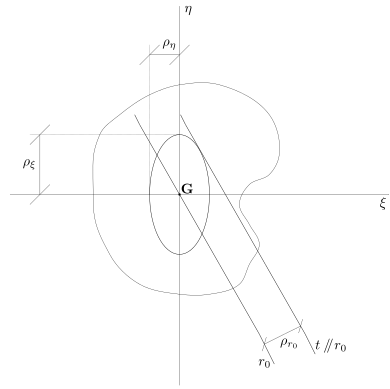
\includegraphics[width=0.75\textwidth]{Immagini/Parte_6/Figura6_1/Figura6_1.pdf}
\caption{}
\label{figura6-1}
\end{figure}
%--------------------------------------------------------------------------------------------------------------------------------------------------------------
Ogni figura piana ha la sua ellisse centrale di inerzia, si veda la figura~\ref{figura6-1}: si tratta dell'ellisse avente il centro coincidente con $\mathbf{G}$, gli assi di simmetria coincidenti con gli assi principali di inerzia $\xi$ ed $\eta$, i raggi principali di lunghezza $\rho_{\xi}$ e $\rho_{\eta}$; da notare che $\rho_{\eta}$ è disteso su $\xi$ e $\rho_{\xi}$ è disteso su $\eta$. In figura~\ref{figura6-1} è anche illustrata un'importante proprietà dell'ellisse di inerzia:
%--------------------------------------------------------------------------------------------------------------------------------------------------------------
\\

\fbox{\begin{minipage}{38em}
\centering
\textsc{Il raggio di inerzia di una figura rispetto ad una retta baricentrica $r_0$ è uguale alla distanza della stessa retta dalla sua parallela $t$ tangente all'ellisse.}
\end{minipage}}
\\
\\

%--------------------------------------------------------------------------------------------------------------------------------------------------------------
\noindent Come è noto dalla \textsc{geometria}, l'ellisse di~\ref{figura6-1} ha equazione
%--------------------------------------------------------------------------------------------------------------------------------------------------------------
\begin{equation} \label{equazione6-2}
\frac{\xi^2}{\rho_{\eta}^{2}}+\frac{\eta^2}{\rho_{\xi}^{2}} = 1
\tag{6.2}
\end{equation}
%--------------------------------------------------------------------------------------------------------------------------------------------------------------
\section{Diametri coniugati di un'ellisse}
%----------------------------------------------------------------------------------------
\renewcommand{\thefigure}{6~-~2}
\begin{figure}[h]
\centering
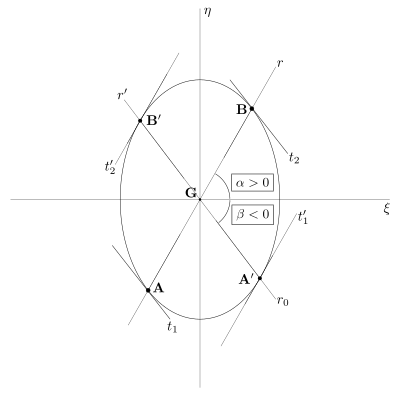
\includegraphics[width=0.75\textwidth]{Immagini/Parte_6/Figura6_2/Figura6_2.pdf}
\caption{}
\label{figura6-2}
\end{figure}
%--------------------------------------------------------------------------------------------------------------------------------------------------------------
Con riferimento alla figura~\ref{figura6-2}, $r$ è un qualunque diametro dell'ellisse ed $\mathbf{A}$ e $\mathbf{B}$ le sue intesezioni; osserviamo intanto che, per una nota proprietà dell'ellisse, le tangenti $t_1$ e $t_2$ sono parallele; $r'$ è il diametro parallelo a $t_1$ e $t_2$, $\mathbf{A}'$ e $\mathbf{B}'$ le sue intersezioni, $t_{1}'$ e $t_{2}'$ le rispettive tangenti. Ebbene, si può dimostrare analiticamente e constatare graficamente che  $t_{1}'$ e $t_{2}'$ sono parallele ad $r$. Ciò premesso, ogni coppia di diametri come $r$ ed $r'$, cioè tali che ognuno è parallelo alle tangenti agli estremi dell'altro, si dicono \textsc{diametri coniugati}. Si potrebbe dimostrare che, per ogni coppia di diametri coniugati, vale la seguente relazione 
%--------------------------------------------------------------------------------------------------------------------------------------------------------------
\begin{equation} \label{equazione6-3}
\boxed{\tan\alpha\cdot\tan\beta = -\frac{I_{\xi}}{I_{\eta}}}
\tag{6.3}
\end{equation}
%--------------------------------------------------------------------------------------------------------------------------------------------------------------
Il segno meno sta ad indicare che gli angoli $\alpha$ e $\beta$ hanno segno opposto, e cioè che i due diametri coniugati stanno sempre in quadranti diversi; in particolare, la figura~\ref{figura6-2}, $\alpha$ è positivo perché antiorario. 
%--------------------------------------------------------------------------------------------------------------------------------------------------------------

\noindent In ogni ellisse esistono chiaramente infinite coppie di diametri coniugati; gli assi principali di inerzia sono l'unica coppia di diametri coniugati \textsc{ortogonali}. Si potrebbe, infine, dimostrare che 
%--------------------------------------------------------------------------------------------------------------------------------------------------------------
\\

\fbox{\begin{minipage}{38em}
\centering
\textsc{Il momento centrifugo è nullo rispetto ad ogni coppia di diametri coniugati.}
\end{minipage}}
\\
\\

%--------------------------------------------------------------------------------------------------------------------------------------------------------------
\noindent In conseguenza di quest'ultima proposizione e in forza del teorema del trasporto del momento centrifugo, è immediato rendersi conto che, se $r_0$ ed $s_0$ sono una qualunque coppia di diametri coniugati, risulta
%--------------------------------------------------------------------------------------------------------------------------------------------------------------
\begin{equation*}
I_{rs_{0}} = I_{r_{0}s} = I_{r_{0}s_{0}} = 0, \qquad \forall r\,\parallelsum r_0 \quad e \quad \forall s\,\parallelsum s_0
\end{equation*}
%--------------------------------------------------------------------------------------------------------------------------------------------------------------
\section{Punti coniugati rispetto all'ellisse}
%----------------------------------------------------------------------------------------
\renewcommand{\thefigure}{6~-~3}
\begin{figure}[ht]
\centering
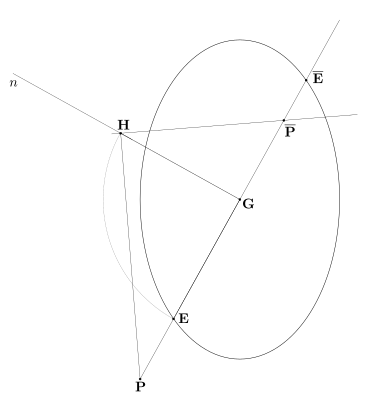
\includegraphics[width=0.75\textwidth]{Immagini/Parte_6/Figura6_3/Figura6_3.pdf}
\caption{}
\label{figura6-3}
\end{figure}
%--------------------------------------------------------------------------------------------------------------------------------------------------------------
Con riferimento alla figura~\ref{figura6-3}, sia $\mathbf{P}$ un punto qualunque del piano; si dice \textsc{coniugato di} $\mathbf{P}$, rispetto all'ellisse, il punto $\overline{\mathbf{P}}$ tale che 
%--------------------------------------------------------------------------------------------------------------------------------------------------------------
\begin{enumerate}
\item $\overline{\mathbf{P}}$ sta sul diametro $\mathbf{P}\mathbf{G}$;
\item $\overline{\mathbf{P}}$ sta dalla parte opposta di $\mathbf{P}$ rispetto a $\mathbf{G}$; 
\item vale la relazione 
%--------------------------------------------------------------------------------------------------------------------------------------------------------------
\begin{equation} \label{equazione6-4}
\lvert\,\mathbf{G}\mathbf{P}\,\lvert\,\lvert\,\mathbf{G}\overline{\mathbf{P}}\,\lvert = \lvert\,\mathbf{G}\mathbf{E}\,\lvert^2
\tag{6.4}
\end{equation}
%--------------------------------------------------------------------------------------------------------------------------------------------------------------
\end{enumerate}
%--------------------------------------------------------------------------------------------------------------------------------------------------------------
In figura~\ref{figura6-3} è illustrata la costruzione $\overline{\mathbf{P}}$
%--------------------------------------------------------------------------------------------------------------------------------------------------------------
\begin{enumerate}
\item si ribalta il raggio $\mathbf{G}\mathbf{E}$ sulla retta $n$ ad esso ortogonale; e dunque $\lvert\,\mathbf{G}\mathbf{H}\,\lvert = \lvert\,\mathbf{G}\mathbf{E}\,\lvert$;
\item si congiunge $\mathbf{P}$ con $\mathbf{H}$ e si traccia da $\mathbf{H}$ la perpendicolare $\mathbf{P}\mathbf{H}$; si interseca così in $\overline{\mathbf{P}}$ la retta $\mathbf{P}\mathbf{G}$.
\end{enumerate}
%--------------------------------------------------------------------------------------------------------------------------------------------------------------
Il secondo teorema di Euclide garantisce che il punto $\overline{\mathbf{P}}$ così determinato verifica la~\eqref{equazione6-4} ed è, pertanto, il coniugato di $\mathbf{P}$. 
%--------------------------------------------------------------------------------------------------------------------------------------------------------------

\noindent Alla luce della~\eqref{equazione6-4} appaiono, infine, ovvie, le seguenti proposizioni
%--------------------------------------------------------------------------------------------------------------------------------------------------------------
\\

\fbox{\begin{minipage}{38em}
\centering
\textsc{Il coniugato di un punto dell'ellisse, come $\mathbf{E}$, è il punto diametralmente opposto $\overline{\mathbf{E}}$.}
\end{minipage}}
\\
\\
%
%%--------------------------------------------------------------------------------------------------------------------------------------------------------------
%\\

\fbox{\begin{minipage}{38em}
\centering
\textsc{Più $\mathbf{P}$ si allontana da $\mathbf{G}$ e più il suo coniugato $\overline{\mathbf{P}}$ i avvicina a $\mathbf{G}$; se $\mathbf{P}$ è fuori dall'ellisse, $\overline{\mathbf{P}}$ si trova all'interno di quest'ultima.}
\end{minipage}}
\\
\\

%--------------------------------------------------------------------------------------------------------------------------------------------------------------
In particolare 
%--------------------------------------------------------------------------------------------------------------------------------------------------------------
\begin{align*}
\mathbf{P} &\rightarrow \infty \iff \overline{\mathbf{P}}\rightarrow \mathbf{G} \\
\mathbf{P} &\rightarrow \mathbf{G} \iff \overline{\mathbf{P}}\rightarrow \infty
\end{align*}
%--------------------------------------------------------------------------------------------------------------------------------------------------------------
\section{Antipolarità rispetto all'ellisse}
%----------------------------------------------------------------------------------------
\renewcommand{\thefigure}{6~-~4}
\begin{figure}[ht]
\centering
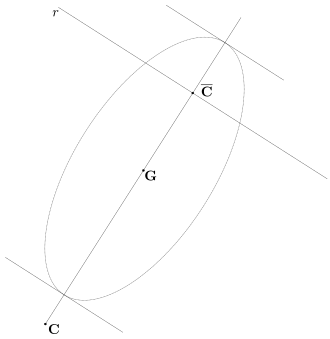
\includegraphics[width=0.75\textwidth]{Immagini/Parte_6/Figura6_4/Figura6_4.pdf}
\caption{}
\label{figura6-4}
\end{figure}
%--------------------------------------------------------------------------------------------------------------------------------------------------------------
Con riferimento alla~\ref{figura6-4}, sia $\mathbf{C}$ un punto e $\overline{\mathbf{C}}$ il suo coniugato; la retta $r$ passante per $\overline{\mathbf{C}}$ e avente direzione coniugata ala diametro $\mathbf{C}\mathbf{G}$ si dice \textsc{antipolare} del punto $\mathbf{C}$ rispetto all'ellisse. Sempre con riferimento alla~\ref{figura6-4}, sia $r$ una generica retta e $\overline{\mathbf{C}}$ l'intersezione di $r$ con il diametro ad essa coniugato; il punto $\mathbf{C}$, coniugato di $\overline{\mathbf{C}}$, si dice \textsc{antipolo} di $r$ rispetto all'ellisse. Resta così definita una corrispondenza fra l'insieme dei punti e l'insieme delle rette del piano
%--------------------------------------------------------------------------------------------------------------------------------------------------------------
\begin{equation*}
\boxed{\textup{\textsc{antipolo}}} \longleftrightarrow \boxed{\textup{\textsc{antipolare}}}
\end{equation*}
%--------------------------------------------------------------------------------------------------------------------------------------------------------------
e tale corrispondenza è chiaramente \textsc{invertibile} e prende il nome di \textsc{antipolarità}. 
%--------------------------------------------------------------------------------------------------------------------------------------------------------------
\noindent Dalla stessa definizione di antipolarità e per una ben nota proprietà dei punti coniugati, scaturisce la seguente proposizione 
%--------------------------------------------------------------------------------------------------------------------------------------------------------------
\\

\fbox{\begin{minipage}{38em}
\centering
\textsc{Più una retta si avvicina a $\mathbf{G}$, più il suo antipolo se ne allontana.}
\end{minipage}}
\\
\\

%--------------------------------------------------------------------------------------------------------------------------------------------------------------
\noindent In particolare: se $r$ passa per $\mathbf{G}$ il suo antipolo sarà il \textsc{punto improprio} in direzione del diametro coniugato ad $r$. 
%--------------------------------------------------------------------------------------------------------------------------------------------------------------

\noindent In geometria si studia che la \textsc{polare} del punto $\mathbf{C}(\xi_{C}, \eta_{C})$ rispetto all'ellisse di equazione~\eqref{equazione6-2} è la retta di equazione 
%--------------------------------------------------------------------------------------------------------------------------------------------------------------
\begin{equation*}
\boxed{\frac{\xi_C}{\rho_{\eta}^{2}}\xi+\frac{\eta_C}{\rho_{\xi}^{2}}\eta -1 = 0}
\end{equation*}
%--------------------------------------------------------------------------------------------------------------------------------------------------------------
In effetti, l'\textsc{antipolare} è la retta \textsc{simmetrica} della polare rispetto all'origine; la sua equazione è pertanto 
%--------------------------------------------------------------------------------------------------------------------------------------------------------------
\begin{equation} \label{equazione6-5}
\boxed{\textup{Equazione dell'antipolare del punto }\mathbf{C}(\xi_{C}, \eta_{C})} \rightarrow \boxed{\frac{\xi_C}{\rho_{\eta}^{2}}\xi+\frac{\eta_C}{\rho_{\xi}^{2}}\eta + 1 = 0}
\tag{6.5}
\end{equation}
%--------------------------------------------------------------------------------------------------------------------------------------------------------------
È dunque immediato, dato un punto, scrivere l'equazione della sua antipolare, e disegnarla rispetto agli assi principali. Ed è pure abbastanza agevole, data una retta $r$, trovare le coordinate del suo antipolo, sempre rispetto agli assi principali; ecco come si procede 
%--------------------------------------------------------------------------------------------------------------------------------------------------------------
\begin{enumerate}
\item si scrive l'equazione di $r$ nella forma 
%--------------------------------------------------------------------------------------------------------------------------------------------------------------
\begin{equation*}
a\xi+b\eta+1=0
\end{equation*}
%--------------------------------------------------------------------------------------------------------------------------------------------------------------
\item dal confronto con la~\eqref{equazione6-5} si ricava immediatamente che 
%--------------------------------------------------------------------------------------------------------------------------------------------------------------
\begin{equation} \label{equazione6-6}
\boxed{\eta_C = a\rho_{\eta}^{2} \quad ; \quad \eta_C = b\rho_{\xi}^{2}}
\tag{6.6}
\end{equation}
%--------------------------------------------------------------------------------------------------------------------------------------------------------------
\end{enumerate}
%--------------------------------------------------------------------------------------------------------------------------------------------------------------
\section{Il nocciolo centrale di inerzia}
%----------------------------------------------------------------------------------------
\renewcommand{\thefigure}{6~-~5}
\begin{figure}[ht]
\centering
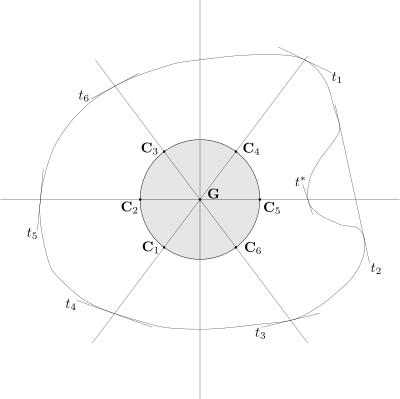
\includegraphics[width=0.75\textwidth]{Immagini/Parte_6/Figura6_5/Figura6_5.pdf}
\caption{}
\label{figura6-5}
\end{figure}
%--------------------------------------------------------------------------------------------------------------------------------------------------------------
\noindent In figura~\ref{figura6-5} è disegnata una generica figura piana; si ritengono noti, anche se non sono stati disegnati, gli assi principali di inerzia $\xi$ ed $\eta$ ed i relativi raggi di inerzia. 
%--------------------------------------------------------------------------------------------------------------------------------------------------------------

\noindent Si pensi alle infinite rette \textsc{tangenti al contorno} ma non secanti la figura: in figura~\ref{figura6-5} se ne sono disegnate soltanto sei; si osservi la retta $t^{*}$: essa, essendo secante la figura, non deve essere annoverata fra le tangenti al contorno.
%--------------------------------------------------------------------------------------------------------------------------------------------------------------

\noindent Di ogni retta tangente, ma non secante, si determini l'antipolo; in figura~\ref{figura6-5} si sono disegnati, solo qualitativamente, gli antipoli $\mathbf{C}_{1},\,\,\mathbf{C}_{2},\,\,\dots\,\,,\,\,\mathbf{C}_{6}$ rispettivamente delle rette $t_{1},\,\,t_{2},\,\,\dots\,\,,\,\,t_{6}$. Se si disegnassero tutti gli antipoli delle infinite rette tangenti, ma non secanti, si otterrebbe una curva, ovviamente chiusa, circondante il baricentro. La zona racchiusa dalla suddetta curva si dice \textsc{nocciolo centrale di inerzia} della figura piana. 
%--------------------------------------------------------------------------------------------------------------------------------------------------------------

\noindent Alla luce di quanto visto nel paragrafo precedente appare ovvia la seguente proposizione 
%--------------------------------------------------------------------------------------------------------------------------------------------------------------
\\

\fbox{\begin{minipage}{38em}
\centering
\textsc{Le rette esterne alla figura hanno antipolo interno al nocciolo e le rette secanti ce l'hanno esterno.}
\end{minipage}}
%--------------------------------------------------------------------------------------------------------------------------------------------------------------
\section{Nocciolo del cerchio}
%----------------------------------------------------------------------------------------
\renewcommand{\thefigure}{6~-~6}
\begin{figure}[ht]
\centering
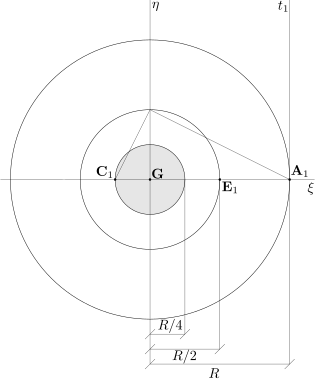
\includegraphics[width=0.51\textwidth]{Immagini/Parte_6/Figura6_6/Figura6_6.pdf}
\caption{}
\label{figura6-6}
\end{figure}
%--------------------------------------------------------------------------------------------------------------------------------------------------------------
\noindent In figura~\ref{figura6-6} è rappresentato un cerchio di raggio $R$. È noto che 
%--------------------------------------------------------------------------------------------------------------------------------------------------------------
\begin{align*}
A &= \pi R^2 \\ 
I_{\xi} &= I_{\eta} = \frac{\pi R^4}{4}
\end{align*}
%--------------------------------------------------------------------------------------------------------------------------------------------------------------
e quindi 
%--------------------------------------------------------------------------------------------------------------------------------------------------------------
\begin{equation*}
\rho_{\xi} = \rho_{\eta} = \frac{R}{2}
\end{equation*}
%--------------------------------------------------------------------------------------------------------------------------------------------------------------
L'ellisse centrale di inerzia del nostro cerchio è, pertanto, ancora un cerchio, ma di raggio $\frac{R}{2}$. 
%--------------------------------------------------------------------------------------------------------------------------------------------------------------

\noindent In figura~\ref{figura6-6} si è costruito l'antipolo $\mathbf{C}_1$ della retta $r_1$: $\mathbf{C}_1$ è ovviamente il coniugato di $\mathbf{A}_1$ e, per definizione di punti coniugati, si veda l'equazione~\eqref{equazione6-4}, risulta 
%--------------------------------------------------------------------------------------------------------------------------------------------------------------
\begin{equation*}
\lvert\,\mathbf{C}_{1}\mathbf{G}\,\lvert = \frac{\lvert\,\mathbf{G}\mathbf{E}_{1}\,\lvert^{2}}{\lvert\,\mathbf{G}\mathbf{A}_{1}\lvert} = \frac{\bigl(\frac{R}{2}\bigr)^2}{R} = \frac{R}{4}
\end{equation*}
%--------------------------------------------------------------------------------------------------------------------------------------------------------------
È immediato convincersi che, per evidenti ragioni di simmetria, tutte le tangenti del cerchio hanno l'antipolo equidistante da $\mathbf{G}$; il nocciolo centrale di inerzia è pertanto un cerchio di raggio $\frac{R}{4}$.
%--------------------------------------------------------------------------------------------------------------------------------------------------------------
\section{Il nocciolo del rettangolo}
%----------------------------------------------------------------------------------------
\renewcommand{\thefigure}{6~-~7}
\begin{figure}[ht]
\centering
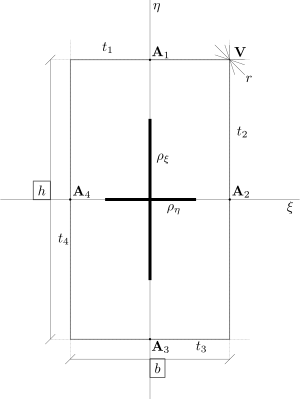
\includegraphics[width=0.51\textwidth]{Immagini/Parte_6/Figura6_7/Figura6_7.pdf}
\caption{}
\label{figura6-7}
\end{figure}
%--------------------------------------------------------------------------------------------------------------------------------------------------------------
\noindent È noto che 
%--------------------------------------------------------------------------------------------------------------------------------------------------------------
\begin{align*}
A &= bh \\ 
I_{\xi} &= \frac{bh^{3}}{12} \\
I_{\eta} &= \frac{b^{3}h}{12}
\end{align*}
%--------------------------------------------------------------------------------------------------------------------------------------------------------------
e dunque 
%--------------------------------------------------------------------------------------------------------------------------------------------------------------
\begin{align*}
\rho_{\xi} &= \frac{h}{\sqrt{12}} \\
\rho_{\eta} &= \frac{b}{\sqrt{12}}
\end{align*}
%--------------------------------------------------------------------------------------------------------------------------------------------------------------
\noindent Abbiamo potuto, così, disegnare i due diametri principali dell'ellisse centrale di inerzia. 
%--------------------------------------------------------------------------------------------------------------------------------------------------------------

\noindent Il contorno del nocciolo è, ovviamente, costituito dagli antipoli delle quattro rette $t_{1}$, $t_{2}$, $t_{3}$ e $t_{4}$, coincidenti con i lati, nonché delle infinite rette come $r$ passanti per i vertici e non secanti. 
%--------------------------------------------------------------------------------------------------------------------------------------------------------------

\noindent L'antipolo $\mathbf{C}_{1}$ di $t_1$ è, ovviamente, il coniugato di $\mathbf{A}_{1}$ e perciò
%--------------------------------------------------------------------------------------------------------------------------------------------------------------
\begin{equation*}
\lvert\,\mathbf{G}\mathbf{C}_{1}\,\lvert = \frac{\rho_{\xi}^{2}}{\lvert\,\mathbf{G}\mathbf{A}_{1}\,\lvert} = \frac{h}{6}
\end{equation*}
%--------------------------------------------------------------------------------------------------------------------------------------------------------------
\noindent L'antipolo $\mathbf{C}_{2}$ di $t_2$ è il coniugato di $\mathbf{A}_{2}$ 
%--------------------------------------------------------------------------------------------------------------------------------------------------------------
\begin{equation*}
\lvert\,\mathbf{G}\mathbf{C}_{2}\,\lvert = \frac{\rho_{\eta}^{2}}{\lvert\,\mathbf{G}\mathbf{A}_{2}\,\lvert} = \frac{b}{6}
\end{equation*}
%--------------------------------------------------------------------------------------------------------------------------------------------------------------
\noindent Gli antipoli $\mathbf{C}_{3}$ e $\mathbf{C}_{4}$ delle rette $t_3$ e $t_4$ sono, ovviamente, i simmetrici di $\mathbf{C}_{1}$ e di $\mathbf{C}_{2}$.
%----------------------------------------------------------------------------------------
\renewcommand{\thefigure}{6~-~8}
\begin{figure}[ht]
\centering
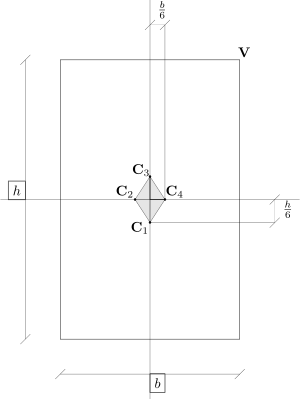
\includegraphics[width=0.51\textwidth]{Immagini/Parte_6/Figura6_8/Figura6_8.pdf}
\caption{}
\label{figura6-8}
\end{figure}
%--------------------------------------------------------------------------------------------------------------------------------------------------------------
Per quanto riguarda gli antipoli delle rette passanti per $\mathbf{V}$, si può dimostrare che essi si trovano sul segmento $\mathbf{C}_{1}\mathbf{C}_{2}$; analogamente, può dirsi per le rette passanti per gli altri vertici. Il nocciolo del rettangolo è, dunque, il \textsc{rombo} le cui diagonali sono lunghe $\frac{1}{3}$ dei lati paralleli, come mostrato in figura~\ref{figura6-8}.
%--------------------------------------------------------------------------------------------------------------------------------------------------------------
\section{Il nocciolo di un profilato}
%--------------------------------------------------------------------------------------------------------------------------------------------------------------
\renewcommand{\thefigure}{6~-~9}
\begin{figure}[ht]
\centering
\subfloat[][]
{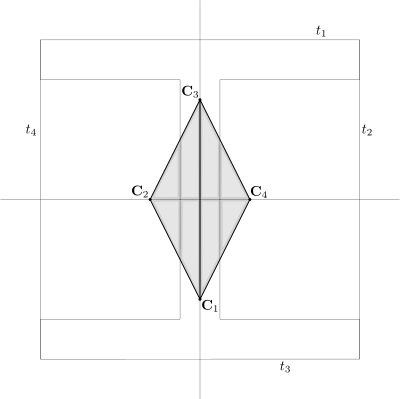
\includegraphics[width=.35\textwidth]{Immagini/Parte_6/Figura6_9/Figura6_9a.pdf}} \quad
\subfloat[][]
{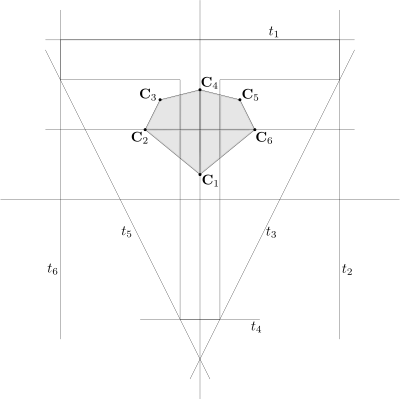
\includegraphics[width=.35\textwidth]{Immagini/Parte_6/Figura6_9/Figura6_9b.pdf}} \\
\subfloat[][]
{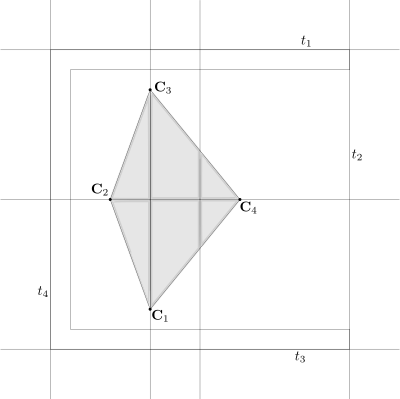
\includegraphics[width=.35\textwidth]{Immagini/Parte_6/Figura6_9/Figura6_9c.pdf}} \quad
\subfloat[][]
{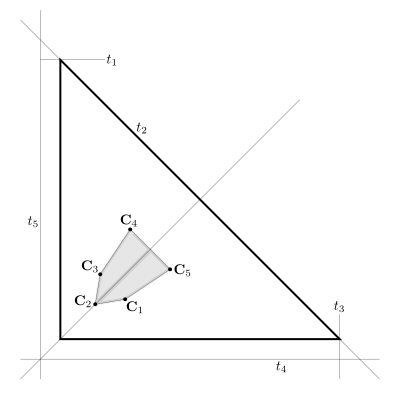
\includegraphics[width=.35\textwidth]{Immagini/Parte_6/Figura6_9/Figura6_9d.pdf}}
\caption{}
\label{figura6-9}
\end{figure}
%--------------------------------------------------------------------------------------------------------------------------------------------------------------
Per disegnare il nocciolo di un profilato occorre e basta determinare gli antipoli di un numero finito di rette, quelle che lambiscono senza intersecare, giacché nei vertici resta valido quanto detto per il rettangolo.
%--------------------------------------------------------------------------------------------------------------------------------------------------------------

\noindent Il nocciolo di un profilato è pertanto un poligono a quattro o più vertici. Nella figura~\ref{figura6-9} sono mostrati, qualitativamente, i noccioli di alcuni fra i tipi più comuni di profilati.
%--------------------------------------------------------------------------------------------------------------------------------------------------------------
\clearpage
\section{Esercizi}
\paragraph{Esercizio 6.1}
Determinare il nocciolo del profilato riportato in figura, dove è disegnata solo la linea media.
%--------------------------------------------------------------------------------------------------------------------------------------------------------------
\renewcommand{\thefigure}{6.1~-~1}
\begin{figure}[ht]
\centering
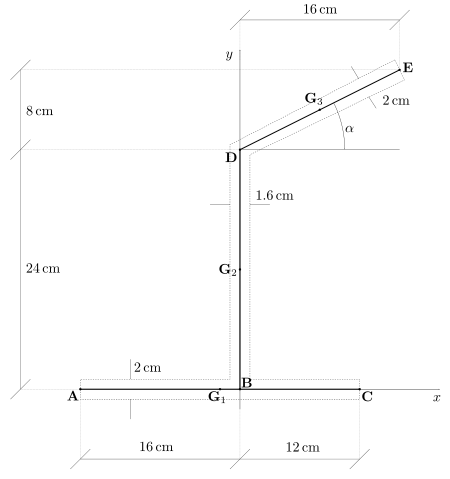
\includegraphics[width=0.75\textwidth]{Immagini/Parte_6/Esercizio6_1/Esercizio6_1_1.pdf}
\caption{}
\label{Esercizio6-1-1}
\end{figure}
%--------------------------------------------------------------------------------------------------------------------------------------------------------------

\noindent Dalla figura si evince che $\tan\alpha=\frac{1}{2}$ e dunque 
%--------------------------------------------------------------------------------------------------------------------------------------------------------------
\begin{align*}
\sin\alpha &= \frac{1}{\sqrt{5}} \\
\cos\alpha &= \frac{2}{\sqrt{5}} \\
\lvert\, DE\,\lvert &= 8\sqrt{5} \approx 17.89\,\textup{cm} \\ 
\alpha &= 25.565^{\circ}
\end{align*}
%--------------------------------------------------------------------------------------------------------------------------------------------------------------
Scelto il riferimento iniziale con assi $x$ ed $y$, calcoliamo le coordinate del baricentro cone note formule
%--------------------------------------------------------------------------------------------------------------------------------------------------------------
%----------------------------------------------------------------------------------------
\begin{equation*}
\begin{aligned}
A_1 &=28\times2 = 56\,\textup{cm}^2 \\
A_2 &=24\times1.6 = 38.400\,\textup{cm}^2 \\
A_3 &=16\sqrt{5} = 35.777\,\textup{cm}^2
\end{aligned}
\,\,\Biggr\}\,\, A = 130.177\,\textup{cm}^2
\end{equation*}
%----------------------------------------------------------------------------------------
\begin{equation*}
\begin{aligned}
S_{1x} &= 0\,\textup{cm}^3 \\
S_{2x} &= 38.4\times12 = 460.800\,\textup{cm}^3 \\
S_{3x} &= 16\sqrt{5}\times 28  = 1001.758\,\textup{cm}^3
\end{aligned}
\,\,\Biggr\}\,\, S_x = 1462.558\,\textup{cm}^3
\end{equation*}
%----------------------------------------------------------------------------------------
\begin{equation*}
\begin{aligned}
S_{1y} &= 56\times(-2) = -112\,\textup{cm}^3 \\
S_{2y} &= 0\,\textup{cm}^3 \\
S_{3y} &= 16\sqrt{5}\times 8  = 286.217\,\textup{cm}^3
\end{aligned}
\,\,\Biggr\}\,\, S_y = 174.217\,\textup{cm}^3
\end{equation*}
%----------------------------------------------------------------------------------------
%--------------------------------------------------------------------------------------------------------------------------------------------------------------
e quindi si ottiene
%--------------------------------------------------------------------------------------------------------------------------------------------------------------
%----------------------------------------------------------------------------------------
\begin{equation*}
\boxed{
x_G = \frac{S_y}{A} = \frac{174.217}{130.177} = 1.338\,\textup{cm}
}
\end{equation*}
%----------------------------------------------------------------------------------------
\begin{equation*}
\boxed{
y_G = \frac{S_x}{A} = \frac{1462.558}{130.177} = 11.235\,\textup{cm}
}
\end{equation*}
%----------------------------------------------------------------------------------------
%--------------------------------------------------------------------------------------------------------------------------------------------------------------
Ora calcoleremo prima $I_x$, $I_y$ e $I_{xy}$ e poi, mediante i teoremi del trasporto, risaliremo ad $I_{x_0}$, $I_{y_0}$ ed $I_{x_{0}y_{0}}$, avendo indicato con $x_0$ ed $y_0$ le rette passanti per $\mathbf{G}$ parallele ad $x$ ed $y$. Conviene, però, fare alcune considerzioni preliminari sul rettangolo $\lvert\,DE\,\lvert$.
%--------------------------------------------------------------------------------------------------------------------------------------------------------------
\renewcommand{\thefigure}{6.1~-~2}
\begin{figure}[ht]
\centering
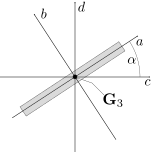
\includegraphics[width=0.53\textwidth]{Immagini/Parte_6/Esercizio6_1/Esercizio6_1_2.pdf}
\caption{}
\label{Esercizio6-1-2}
\end{figure}
%--------------------------------------------------------------------------------------------------------------------------------------------------------------
\begin{align*}
I_a &= \frac{8\sqrt{5}\times2^{3}}{12} = 12\,\textup{cm}^4 \\
I_b &= \frac{2\times(8\sqrt{5})^{3}}{12} = 954\,\textup{cm}^4
\end{align*}
%--------------------------------------------------------------------------------------------------------------------------------------------------------------
Ora valuteremo $I_c$, $I_d$ e $I_{cd}$ applicando le formule di trasformazione~\eqref{equazione4-1} ponendo in esse $\varphi=-\alpha$ ed identificando $I_x$ con $I_a$, $I_y$ con $I_b$ ed $I_{xy}$ con $I_{ab}=0$. Abbiamo dunque 
%--------------------------------------------------------------------------------------------------------------------------------------------------------------
\begin{align*}
\sin^{2}\varphi &= \sin^{2}\alpha = \frac{1}{5} \\
\cos^{2}\varphi &= \cos^{2}\alpha = \frac{4}{5} \\ 
\sin2\varphi &= -\sin2\alpha = -2\sin\alpha\cos\alpha = -2\frac{1}{\sqrt{5}}\frac{2}{\sqrt{5}} = -\frac{4}{5}
\end{align*}
%--------------------------------------------------------------------------------------------------------------------------------------------------------------
\begin{align*}
I_c &= I_{a}\cos^{2}\varphi+I_{b}\sin^{2}\varphi = 12\frac{4}{5}+954\frac{1}{5} = 200\,\textup{cm}^4 \\
I_d &= I_{a}\sin^{2}\varphi+I_{b}\cos^{2}\varphi = 12\frac{1}{5}+954\frac{4}{5} = 766\,\textup{cm}^4 \\
I_{cd} &= \frac{I_{a}-I_{b}}{2}\sin2\varphi = \frac{12-954}{2}\biggl(-\frac{4}{5}\biggr) = 377\,\textup{cm}^4
\end{align*}
%--------------------------------------------------------------------------------------------------------------------------------------------------------------
Ed ora passiamo al calcolo di $I_x$, $I_y$ e $I_{xy}$:
%--------------------------------------------------------------------------------------------------------------------------------------------------------------
%----------------------------------------------------------------------------------------
\begin{equation*}
\begin{aligned}
I_{1x} &= \frac{28\times2^{3}}{12} = 19\,\textup{cm}^4 \\
I_{2x} &= \frac{1.6\times24^{3}}{3} = 7373\,\textup{cm}^4 \\
I_{3x} &= I_c+A_{3}y_{G_3}^{2} = 200+16\sqrt{5}\times28^2 = 28249\,\textup{cm}^4 
\end{aligned}
\,\,\Biggr\}\,\, I_x = 35641\,\textup{cm}^4
\end{equation*}
%----------------------------------------------------------------------------------------
\begin{equation*}
\begin{aligned}
I_{1y} &= \frac{2\times28^{3}}{12} + 56\times2^2= 3883\,\textup{cm}^4 \\
I_{2y} &= \frac{24\times1.6^{3}}{12} = 8\,\textup{cm}^4 \\
I_{3y} &= I_d+A_{3}x_{G_3}^{2} = 766+16\sqrt{5}\times8^2 = 3056\,\textup{cm}^4 
\end{aligned}
\,\,\Biggr\}\,\, I_y = 6947\,\textup{cm}^4
\end{equation*}
%----------------------------------------------------------------------------------------
\begin{equation*}
\begin{aligned}
I_{1xy} &= 0 \\
I_{2xy} &= 0 \\
I_{3xy} &= I_{cd}+A_{3}x_{G_3}y_{G_3} = 377 + 16\sqrt{5}\times8\times28 = 8391\,\textup{cm}^4 
\end{aligned}
\,\,\Biggr\}\,\, I_y = 8391\,\textup{cm}^4
\end{equation*}
%----------------------------------------------------------------------------------------
%--------------------------------------------------------------------------------------------------------------------------------------------------------------
E finalmente calcoliamo  $I_{x_{0}}$, $I_{y_{0}}$ e $I_{x_{0}y_{0}}$
%--------------------------------------------------------------------------------------------------------------------------------------------------------------
\begin{align*}
I_{x_{0}} &= I_x - Ay_{G}^{2} = 35641-130.177\times11.235^{2} = 19209\,\textup{cm}^4 \\
I_{y_{0}} &= I_y - Ax_{G}^{2} = 6947-130.177\times1.338^{2} = 6714\,\textup{cm}^4 \\
I_{x_{0}y_{0}} &= I_{xy}-Ax_{G}y_{G} = 8391-130.177\times1.338\times11.235 = 6434\,\textup{cm}^4
\end{align*}
%--------------------------------------------------------------------------------------------------------------------------------------------------------------
Ora calcoliamo l'angolo $\varphi^{*}=\widehat{\xi x_{0}}$ 
%--------------------------------------------------------------------------------------------------------------------------------------------------------------
\begin{equation*}
\tan2\varphi^{*}=\frac{2I_{x_{0}y_{0}}}{I_{y_{0}}-I_{x_{0}}} = \frac{2\times6434}{6714-19209} \longrightarrow \tan2\varphi^{*}=-1.02985
\end{equation*}
%--------------------------------------------------------------------------------------------------------------------------------------------------------------
e dunque 
%--------------------------------------------------------------------------------------------------------------------------------------------------------------
\begin{equation*}
2\varphi^{*} = -45.84^{\circ} \longrightarrow \boxed{\varphi^{*}=-22.92^{\circ}}
\end{equation*}
%--------------------------------------------------------------------------------------------------------------------------------------------------------------
I valori di $I_{\xi}$ ed $I_{\eta}$ si possono ottenere utilizzando la~\eqref{equazione5-2a} come segue
%--------------------------------------------------------------------------------------------------------------------------------------------------------------
\begin{equation*}
\begin{aligned}
I_{\xi} & \\
I_{\eta} &
\end{aligned}
\,\,\Biggr\}\,\, \frac{I_{x}+I_{y}}{2} \pm \sqrt{\biggl(\frac{I_{x}-I_{y}}{2}\biggr)^{2}+I_{xy}^{2}}=12961\pm8968
\end{equation*}
%--------------------------------------------------------------------------------------------------------------------------------------------------------------
e quindi
%--------------------------------------------------------------------------------------------------------------------------------------------------------------
\begin{align*}
I_{\xi} &= 21929\,\textup{cm}^{4} \\
I_{\eta} &= 3993\,\textup{cm}^{4}
\end{align*}
%--------------------------------------------------------------------------------------------------------------------------------------------------------------
I raggi principali di inerzia valgono, dunque
%--------------------------------------------------------------------------------------------------------------------------------------------------------------
\begin{align*}
\rho_{\xi}^{2} &= \frac{I_{\xi}}{A} = \frac{21929}{130.177} = 168.455\,\textup{cm}^{2} \\
\rho_{\eta}^{2} &= \frac{I_{\eta}}{A} = \frac{3993}{130.177} = 30.674\,\textup{cm}^{2}
\end{align*}
%--------------------------------------------------------------------------------------------------------------------------------------------------------------
Il nocciolo del nostro profilato avrà per vertici gli antipoli delle rette $\mathbf{A}\mathbf{C}$, $\mathbf{A}\mathbf{D}$, $\mathbf{C}\mathbf{E}$, $\mathbf{D}\mathbf{E}$ e sarà, pertanto, un quadrilatero.
%--------------------------------------------------------------------------------------------------------------------------------------------------------------
Ricaveremo le coordinate degli antipoli delle quattro rette suddette utilizzando le~\eqref{equazione6-5}. Naturalmente dobbiamo scrivere le equazioni delle quattro rette suddette nel riferimento $\mathbf{G}\xi\eta$; e, a tale scopo, abbiamo bisogno delle coordinate dei punti $\mathbf{A}$, $\mathbf{C}$, $\mathbf{D}$, $\mathbf{E}$ nello stesso riferimento. Intanto, nel riferimento $\mathbf{G}x_{0}y_{0}$ i punti in questione hanno coordinate
%--------------------------------------------------------------------------------------------------------------------------------------------------------------
\begin{align*}
x_{0A} &= -17.338\,\textup{cm} \\ 
y_{0A} &= -11.235\,\textup{cm} 
\end{align*}
%--------------------------------------------------------------------------------------------------------------------------------------------------------------
\begin{align*}
x_{0D} &= -1.338\,\textup{cm} \\ 
y_{0D} &= 12.765\,\textup{cm} 
\end{align*}
%--------------------------------------------------------------------------------------------------------------------------------------------------------------
\begin{align*}
x_{0C} &= 10.662\,\textup{cm} \\ 
y_{0C} &= -11.235\,\textup{cm} 
\end{align*}
%--------------------------------------------------------------------------------------------------------------------------------------------------------------
\begin{align*}
x_{0E} &= 14.662\,\textup{cm} \\ 
y_{0E} &= 20.765\,\textup{cm} 
\end{align*}
%--------------------------------------------------------------------------------------------------------------------------------------------------------------
Nel riferimento $\mathbf{G}\xi\eta$, le coordinate dei quattro punti in questione si possono ricavare mediante le formule di trasformazione delle coordinate
%--------------------------------------------------------------------------------------------------------------------------------------------------------------
\begin{align*}
\xi &= x_{0}\cos\varphi^{*}+y_{0}\sin\varphi^{*} \\ 
\eta &= -x_{0}\sin\varphi^{*}+y_{0}\cos\varphi^{*}
\end{align*}
%--------------------------------------------------------------------------------------------------------------------------------------------------------------
Nella fattispecie, daremo le coordinate dei punti $\mathbf{C}_2$ e $\mathbf{C}_3$. Si ha
%--------------------------------------------------------------------------------------------------------------------------------------------------------------
\begin{equation*}
r_2 \longrightarrow \frac{28.336}{236.358}\xi - \frac{5.390}{236.358}\eta + 1 = 0
\end{equation*}
%--------------------------------------------------------------------------------------------------------------------------------------------------------------
e dunque le coordinate di $\mathbf{C}_2$ sono 
%--------------------------------------------------------------------------------------------------------------------------------------------------------------
\begin{align*}
\xi_{C_{2}} &= \frac{28.336}{236.358}30.674 = 3.617\,\textup{cm} \\ 
\eta_{C_{2}} &= -\frac{5.390}{236.358}168.455 = -3.841\,\textup{cm}
\end{align*}
%--------------------------------------------------------------------------------------------------------------------------------------------------------------
Passiamo alla retta $CE = r_3$ 
%--------------------------------------------------------------------------------------------------------------------------------------------------------------
\begin{equation*}
r_3 \longrightarrow (\xi - 14.196)31.032 = (\eta+6.196)(-8.779)
\end{equation*}
%--------------------------------------------------------------------------------------------------------------------------------------------------------------
E dunque 
%--------------------------------------------------------------------------------------------------------------------------------------------------------------
\begin{equation*}
r_3 \longrightarrow -\frac{31.032}{386.135}\xi - \frac{8.779}{386.135}\eta + 1 = 0
\end{equation*}
%--------------------------------------------------------------------------------------------------------------------------------------------------------------
e dunque le coordinate di $\mathbf{C}_3$ sono 
%--------------------------------------------------------------------------------------------------------------------------------------------------------------
\begin{align*}
\xi_{C_{3}} &= -\frac{31.032}{386.135}30.674 = -2.465\,\textup{cm} \\ 
\eta_{C_{3}} &= -\frac{8.779}{386.135}168.455 = -3.830\,\textup{cm}
\end{align*}
%--------------------------------------------------------------------------------------------------------------------------------------------------------------
\renewcommand{\thefigure}{6.1~-~3}
\begin{figure}[ht]
\centering
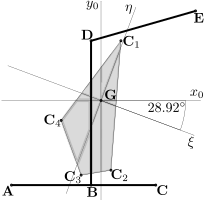
\includegraphics[width=\textwidth]{Immagini/Parte_6/Esercizio6_1/Esercizio6_1_3.pdf}
\caption{}
\label{Esercizio6-1-3}
\end{figure}
%--------------------------------------------------------------------------------------------------------------------------------------------------------------
Il nocciolo della nostra figura è riportato in figura~\ref{Esercizio6-1-3}.
%--------------------------------------------------------------------------------------------------------------------------------------------------------------